\documentclass[12pt, twoside]{article}
\usepackage[letterpaper, margin=1in, headsep=0.5in]{geometry}
\usepackage[english]{babel}
\usepackage[utf8]{inputenc}
\usepackage{amsmath}
\usepackage{amsfonts}
\usepackage{amssymb}
\usepackage{tikz}
%\usetikzlibrary{quotes, angles}

\usepackage{graphicx}
\usepackage{enumitem}
\usepackage{multicol}

\usepackage{fancyhdr}
\pagestyle{fancy}
\fancyhf{}
\renewcommand{\headrulewidth}{0pt} % disable the underline of the header

\fancyhead[R]{\thepage}
\fancyhead[L]{BECA / Dr. Huson / 10th Grade Geometry\\* Learning trajectory: Transformations}

\begin{document}
\subsubsection*{Transformations}
  \begin{enumerate}
  \item Translations with alternate notations
  \item Corresponding angles, points, sides after rigid tranformations
  \item Use in proofs
  \begin{enumerate}
    \item Reflection or rotation of a line segment
    \item Rigid
    \item Triangle midlines
    \item Notation, standard "justify" language
    \end{enumerate}
  \item Dilation impact on lengths, area, angles (volume)
  \end{enumerate}

  \begin{enumerate}
    \subsubsection*{Translations}
    \item Calculating results as coordinate pairs
    \item Prime notation
    \item Multiple transformations

    \item Triangle $A'B'C'$ is the image of triangle $ABC$ after a translation of 2 units to the right and 3 units up. Is triangle $ABC$ congruent to tirangle $A'B'C'$ ? Explain why.

    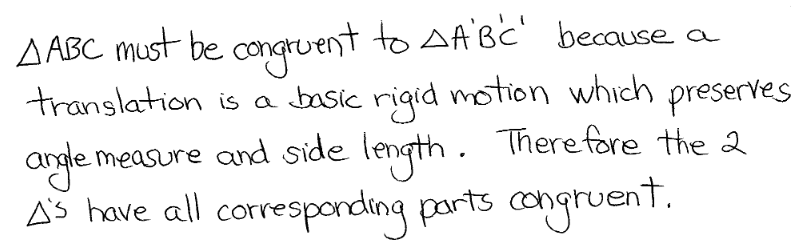
\includegraphics[width=0.9\textwidth]{Isometry_JN2018-25-sol.png}\\
    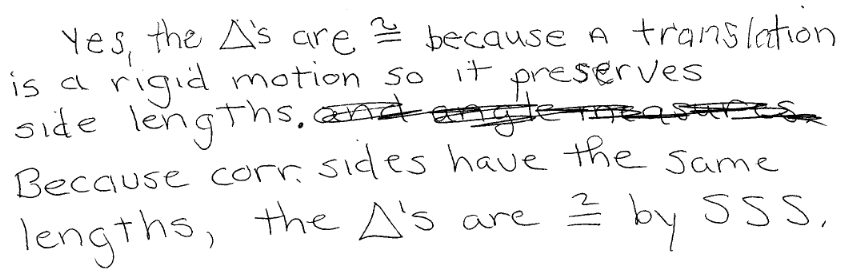
\includegraphics[width=0.9\textwidth]{Isometry_JN2018-25-sol2.png}

    \item Symmetry: If when an object $A \rightarrow A'$ and $A = A'$ then we say it is symmetric. \\
    Reflection: \emph{axis of symmetry}\\
    Rotation: \emph{center and angle of rotation}\\[0.25cm]
    Example: Regular polygons are symmetrical\\[0.25cm]

    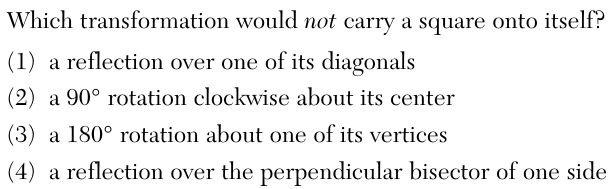
\includegraphics[width=0.7\textwidth]{symmetry-square_JA2018-15.png}\\[0.5cm]
    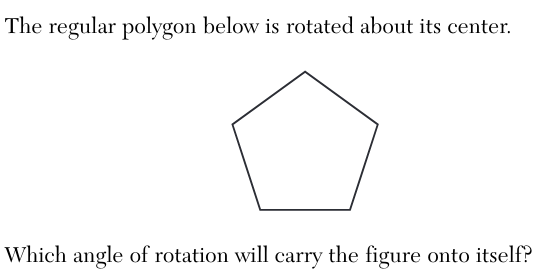
\includegraphics[width=0.7\textwidth]{symmetry_JN2018-19.png}

  \end{enumerate}

\end{document}
